\section{Query Evaluation}
\label{sec:result_generation}


The more nodes we insert in the $kd$-tree the more complicated it is to find the qualifying tuples.
There might be four different kinds of partitions indicated by the $kd$-tree nodes.
\begin{itemize}
\item Partitions that can be entirely omitted from the result
\item Partitions that are entirely included in the result
\item Partitions that are partially included in the result and must be cracked further
\item Partitions that are partially included in the result and have to be scanned
\end{itemize}
We need an efficient algorithm to decide and deal with different partitions in order to return the correct result.

Figure~\ref{fig:kdtree_big} shows a $kd$-tree with many nodes.
This is a better example to show how our algorithms work.
The main problem with such a big $kd$-tree is that we cannot show nicely how the data is reorganized, but hopefully the reader will get the idea if they are familiar with database cracking or if they understand the first two examples.

%\begin{figure}[]
%   \begin{center}
%   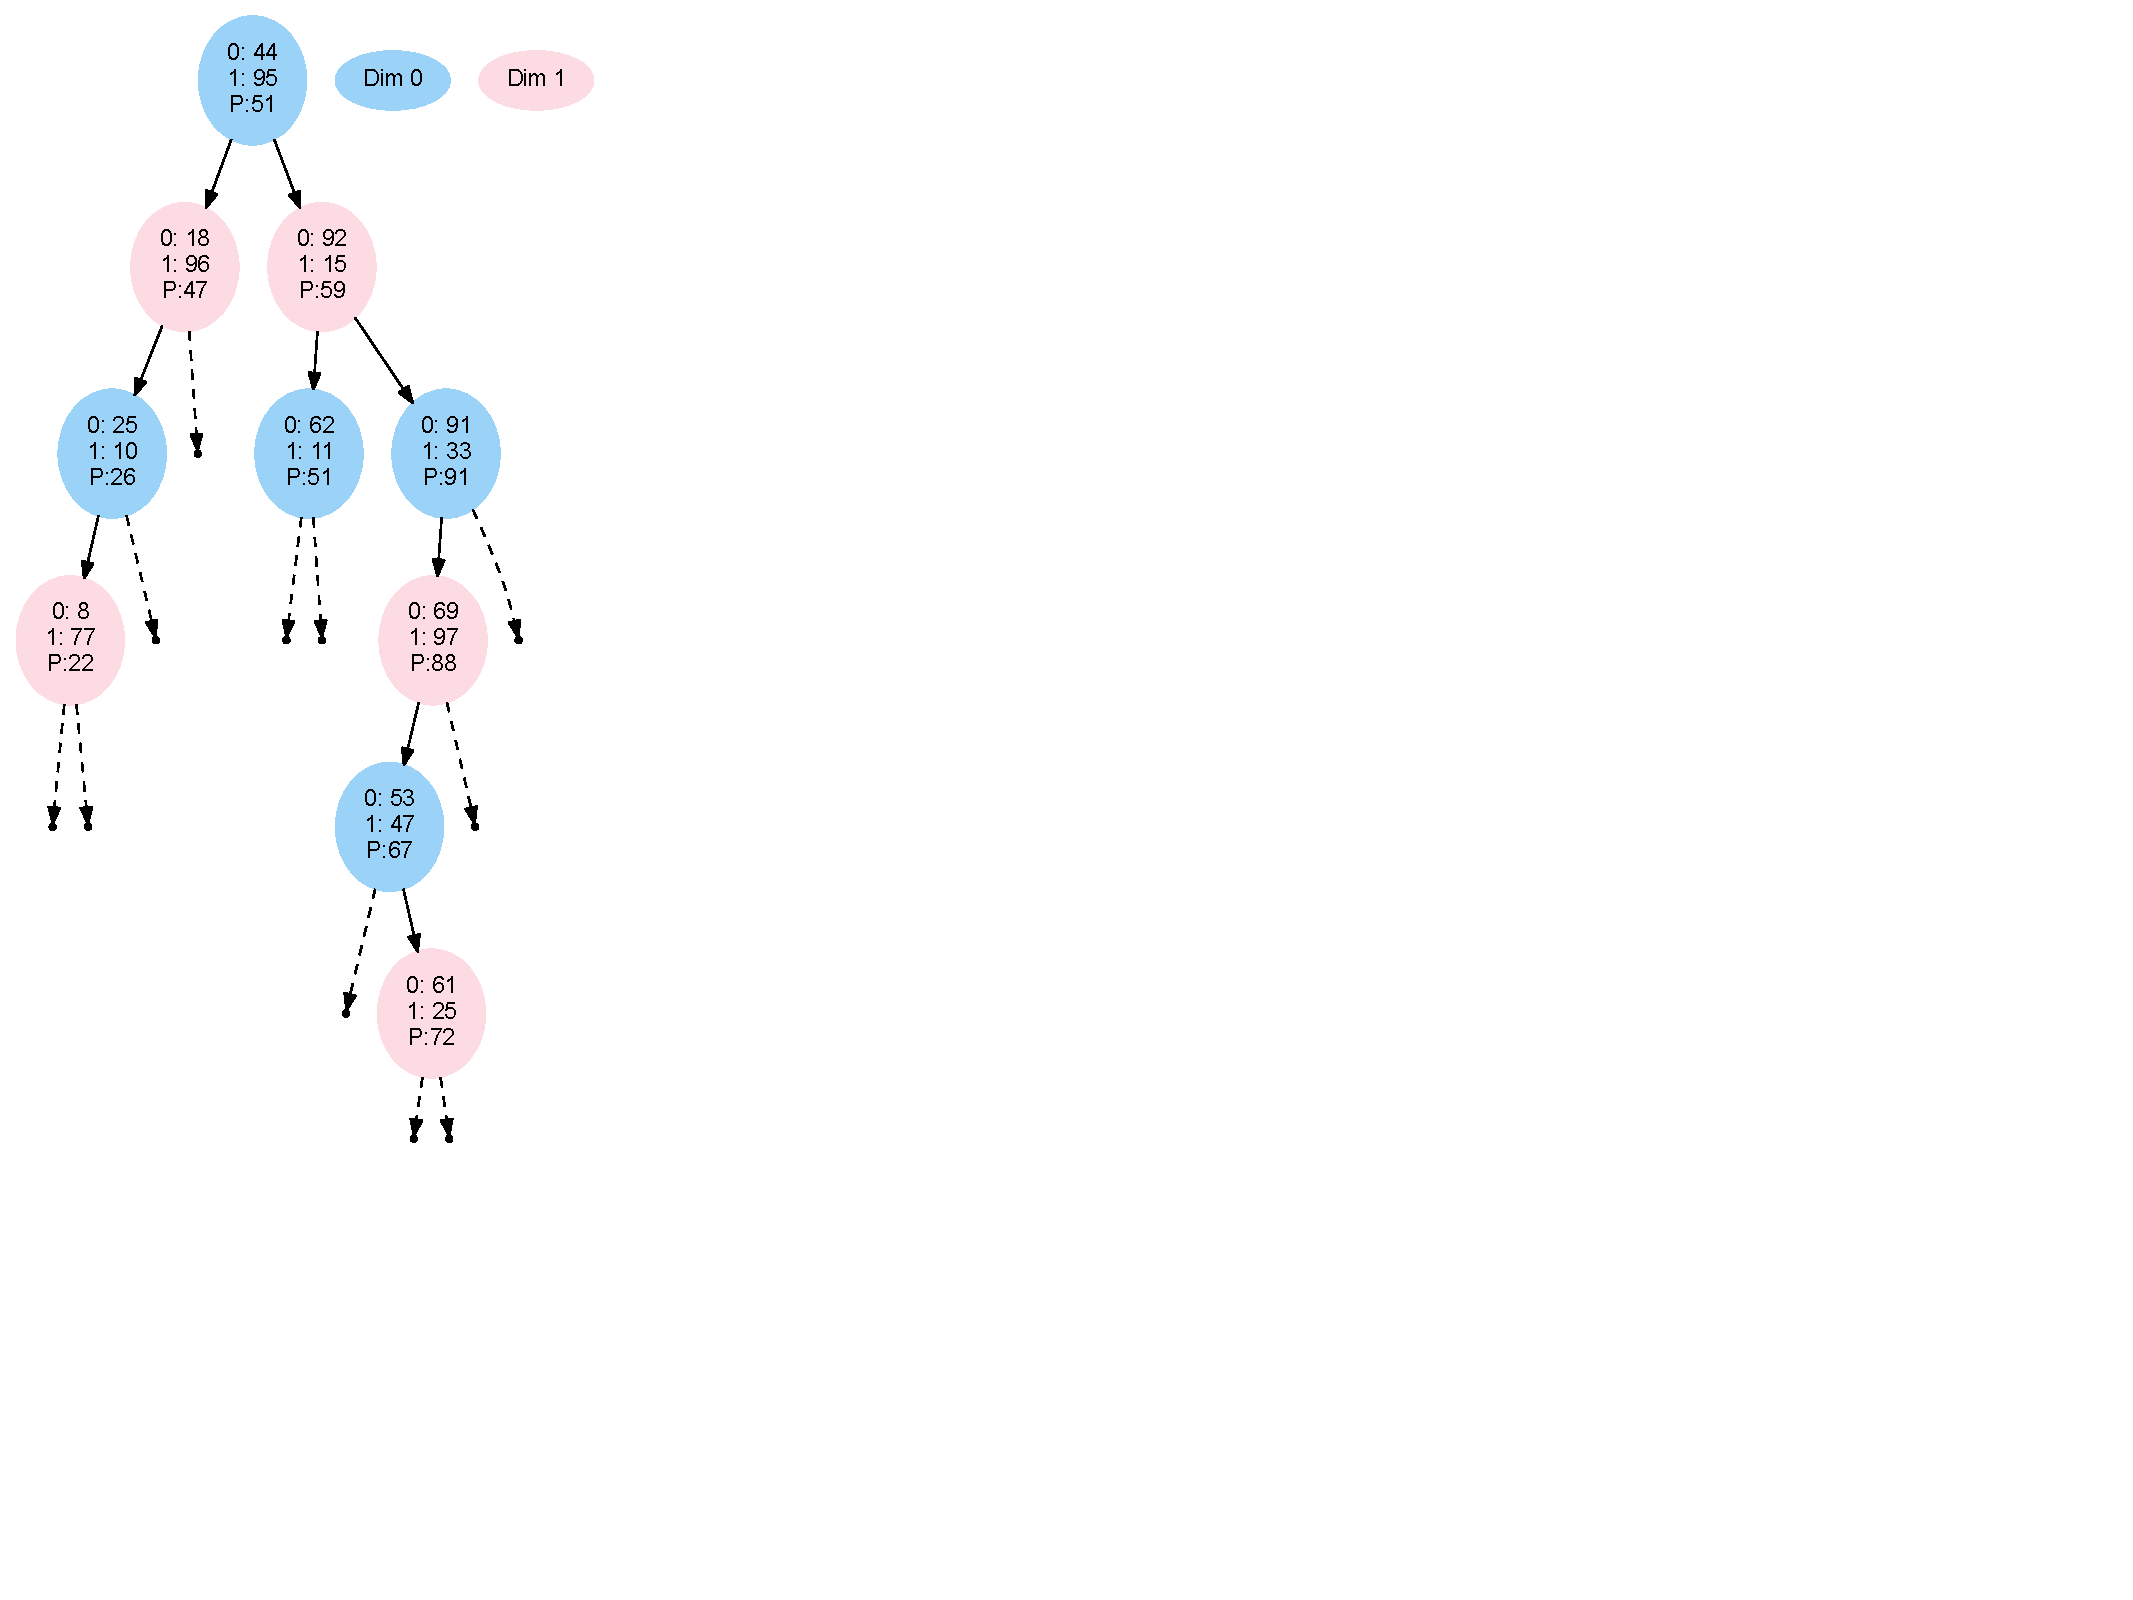
\includegraphics[trim=0cm 8cm 14cm 0cm,width=0.9\textwidth]{Figures/kdtree_big}
%   \caption{2nd crack on 8 $2$-dimensional points.}
%   \label{fig:kdtree_big}
%   \end{center}
%\end{figure}


\subsection{Query Types}
\label{subsec:queries}

%Data filtering, i.e., retrieval of a subset of records that qualify for the selection predicates of a given query, is the most common operation in database systems.
%Selection predicates might vary from very simple predicates such as $\mathtt{\{P|K_2(P)=10\}}$ to complex sets such as $\mathtt{\{P|[(1 \leq K_1(P) < 10) \vee (K_2(P) < 20) \wedge (K_3(P) = 5)]\}}$.
%We classify selection queries as a) exact match queries, b) partial match queries and c) region queries.
%Each query type needs a different search strategy \cite{Bentley:1975:MBS:361002.361007}.
%In this section we present how we adjust the search strategies to the requirements of adaptive clustering.

%\textbf{Exact Match Queries.} Exact match queries retrieve specific records, i.e., they search for records $\mathtt{r}$ that qualify the following condition.
%\begin{center}
%$\mathtt{\{r|K_i(r)=v_i for 0 \leq i < k\}}$ 
%\end{center}

%\textbf{Partial Match Queries.} Partial match queries search for a subset of $\mathtt{t}$ keys out of $\mathtt{k}$ keys that are stored in the $kd$-tree.
%Assuming that $\mathtt{\{s_i\}}$ and $\mathtt{\{v_i\}}$ are sets such that the keys specified are $\mathtt{K_{s_0}, K_{s_1}, \dots, K_{s_t}}$ and the values they must have to be a valid response to the query are $\mathtt{v_{s_0}, v_{s_1}, \dots, v_{s_t}}$, we search for records that qualify the following condition.
%\begin{center}
%$\mathtt{\{r|K_{s_i}(r)=v_{s_i} for 0 \leq i < t\}}$ 
%\end{center}
%We use the $kd$-tree to navigate to the correct partition(s). Every time we visit a node $\mathtt{P}$, we check if the node satisfies the query predicates.
%Let $\mathtt{j}$ be the discriminator $\mathtt{DISC(P)}$ of $\mathtt{P}$.
%If $\mathtt{j=s_i}$ for some $\mathtt{i}$, then we continue our search to one of the subtrees of $\mathtt{P}$; if $\mathtt{v_{s_i} < K_j(P)}$ we continue to $\mathtt{LEFT(P)}$, else if $\mathtt{v_{s_i} > K_j(P)}$ we continue to $\mathtt{RIGHT(P)}$.
%If $\mathtt{j \notin \{s_i\}}$ then we continue the search in both subtrees. 

%\textbf{Region Queries.} This is the most generic type of selection queries. It searches for all records that intersect with a given range.
%To accomplish a search of the qualifying records, we need to find two types of partitions; a) partitions that are entirely included in the result and b) partitions that intersect with the result, but they might contain values that do not qualify the query.
%The \emph{bounds array} is necessary here in order to determine the bounds of each partition.



